\section{Ergebnisse}

Um einen guten Klassfizierer zu bekommen, waren einige Trainingsdurchläufe notwendig. So kamen wir letzten Endes auf etwa 30 Trainingsdurchläufe, die jeweils einige Tage trainierten. Zur Parameteroptimierung für das Training wurden die trainierten Klassifizierer auf einen Validierungs-Datensatz angewandt, wobei die ersten Durchgänge dabei nur minimal bessere Ergebnisse als der Zufall lieferten. Durch verschiedene Anpassungen, die in Kapitel~\ref{training} näher erläutert wurden, konnten schließlich besser Ergebnisse erzielt werden. 


\begin{figure}[htb!]
	\centering
	\begin{subfigure}[t]{0.49\textwidth}
		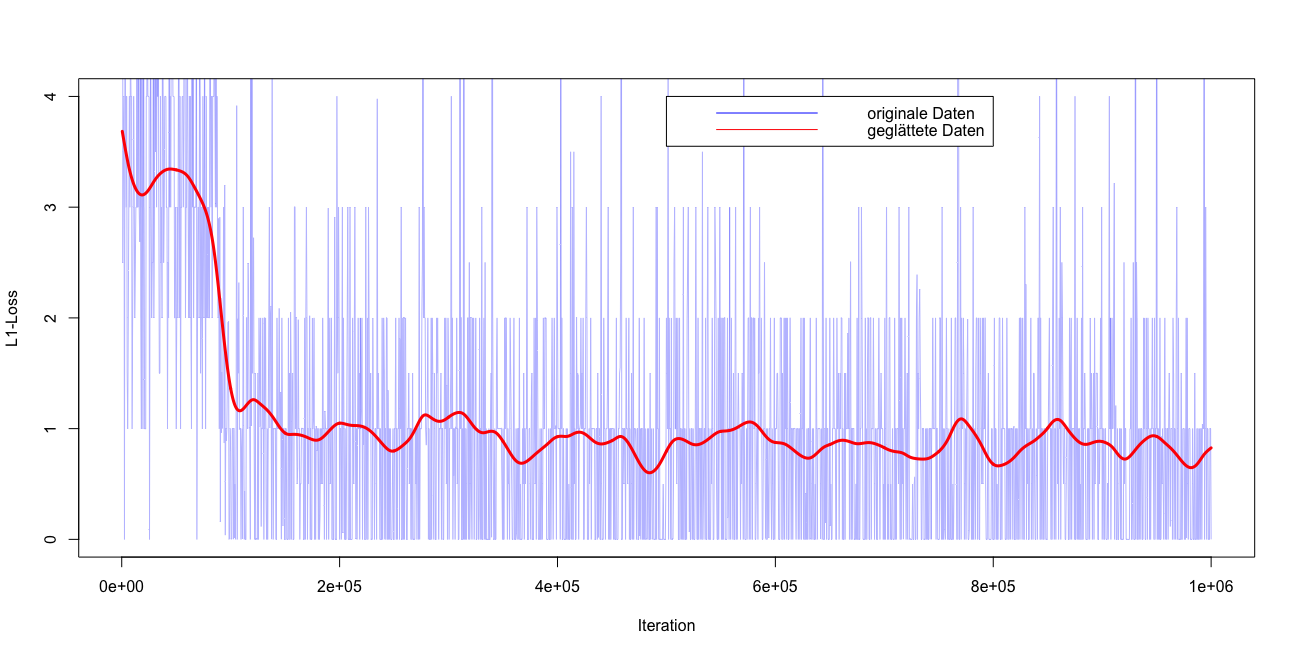
\includegraphics[width=\textwidth]{pics/losses/l1_loss.png}
		\caption{L1-Loss}
		\label{fig:losses_l1}
	\end{subfigure}
	\hfill
	\begin{subfigure}[t]{0.49\textwidth}
		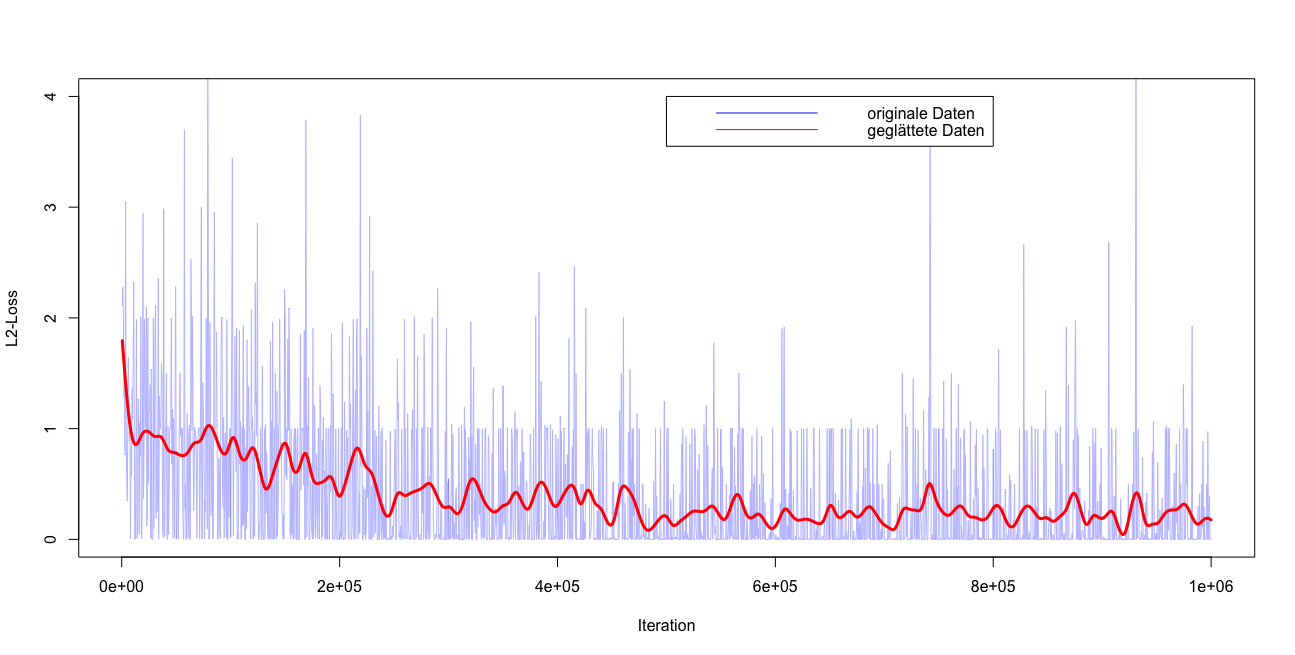
\includegraphics[width=\textwidth]{pics/losses/l2_loss.png}
		\caption{L2-Loss}
		\label{fig:losses_l2}
	\end{subfigure}
	\hfill
	\begin{subfigure}[t]{0.49\textwidth}
		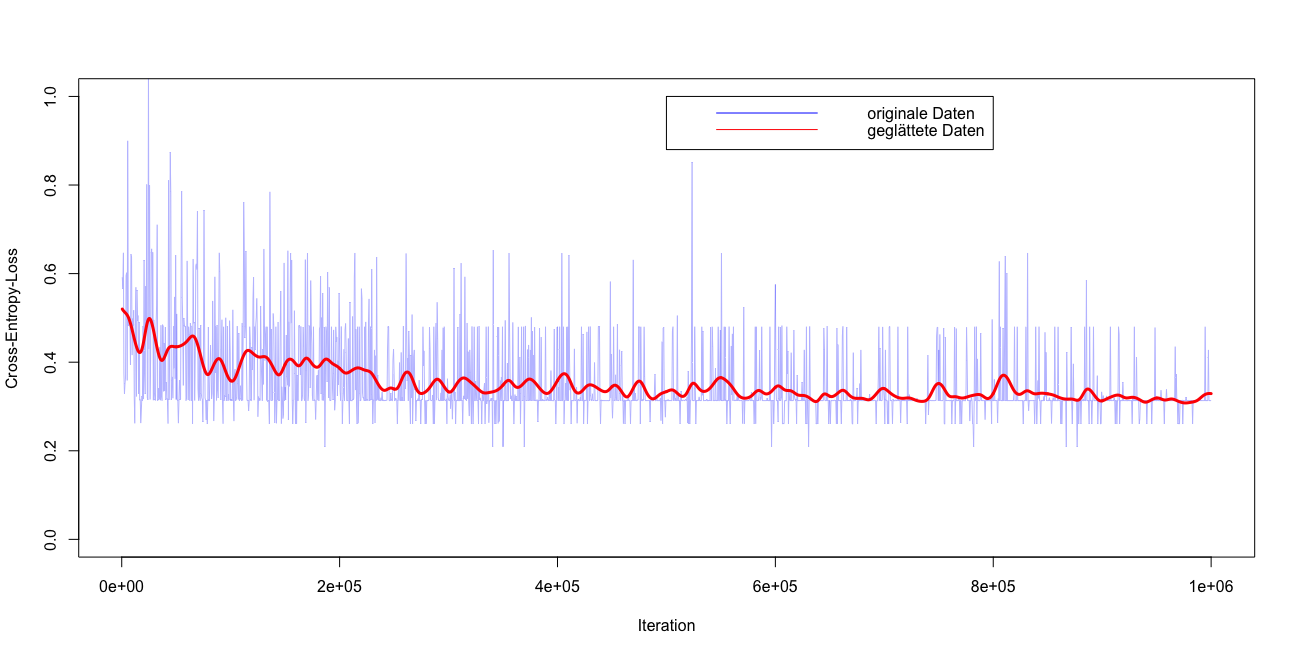
\includegraphics[width=\textwidth]{pics/losses/ce_loss.png}
		\caption{Softmax-Kreuzentropie-Loss}
		\label{fig:losses_ce}
	\end{subfigure}		
	\caption{Konvergenzverhalten verschiedener Loss-Funktionen bei gleichen Trainingsparametern.}
	\label{fig:losses}			
\end{figure}

Einen großen Einfluss auf das Training hatte die Wahl der Loss-Funktion. Aus diesem Grund haben wir die Funktionen anfangs mit Blick auf ihr Konvergenzverhalten bei unserem Klassifizierungsansatz untersucht. In Abbildung \ref{fig:losses} sind die in Kapitel \ref{training} besprochenen Loss-Funktionen über den Verlauf je eines Trainings gezeigt. Dabei fällt auf, dass der L1-Loss (Abbildung \ref{fig:losses_l1}) anfangs stark abfällt, jedoch nach etwa $100000$ Iterationen stagniert. Betrachtet man hingegen die Kurve des L2-Loss (Abbildung \ref{fig:losses_l2}), ist ein kontinuierlicher Abfall des Losses über eine deutlich längere Zeit (bis etwa Iteration $600000$) erkennbar. Eine längere Trainingsphase verbessert die Performanz des Trainierten Netzes. Die Gewichte des Netzes können so besser trainiert werden. Im Vergleich dazu ändert sich der Softmax-Kreuzentropie-Loss (Abbildung \ref{fig:losses_ce}) kaum. Der Wert dieser Loss-Funktion ändert sich kaum. Dadurch ist für das Training unseres neuronalen Netzes ein nur wenig aussagekräftiger Gradient verfügbar. Somit scheint der L2-Loss die am besten geeignete Loss-Funktion für unsere Problemstellung zu sein. Dies zeigte sich auch bei der Evaluation der Netze.\\

Unser erfolgreichstes Training (2018-03-10\_19-16-32) wurde mit einem L2-Loss und einer Lernrate von $\eta= 0.000001$ trainiert. Die Ergebnisse einiger ausgewählter Trainingsdurchläufe werden in Abbildung~\ref{fig:roc} als ROC-Kurve dargestellt. Jede Kurve steht für einen ausgewählten Klassifizierer und die entsprechende Anwendung auf den Validierungsdatensatz. Wie man gut erkennen kann, verlaufen zwei der Kurven nahe der Diagonalen. Die beiden Klassifikator (2018-03-12\_22-04-38 und 2018-03-12\_22-17-46) liefern somit keine guten Ergebnisse und sind nur etwas besser als eine zufällige Entscheidung. Gute Klassifikatoren verlaufen in der ROC-Kurve links oben und sind in diesem Fall 2018-03-10\_19-16-32, 2018-03-09\_21-34-4 und 2018-04-13\_20-38-20. Die anderen Klassifikatoren können auf den ersten Blick als in Ordnung eingestuft werden.

\begin{figure}[htb!]
	\begin{center}
		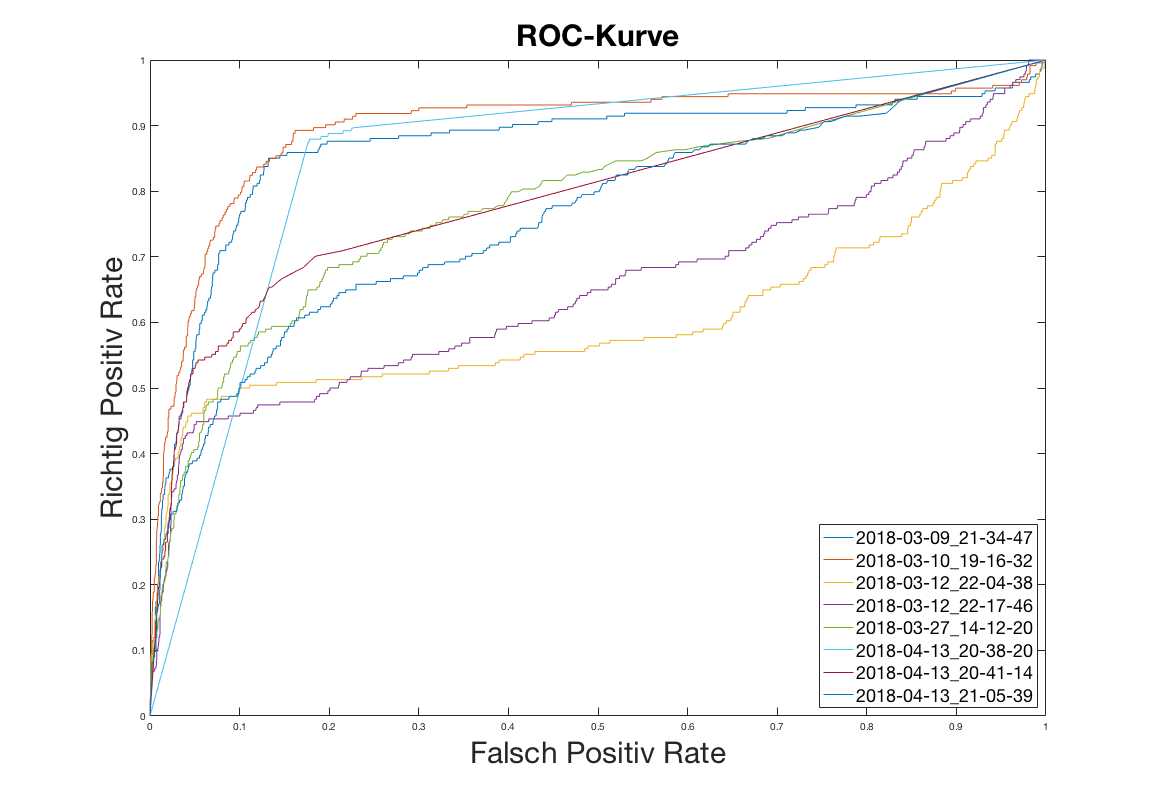
\includegraphics[width=0.8\textwidth]{pics/evaluation/roc_analysis.png}
		\caption{ROC-Kurven einiger trainierter Klassifizierer, angewandt auf den Validierungs-Datensatz.}
		\label{fig:roc}
    \end{center}
\end{figure}

Um die ROC-Kurve nicht nur optisch, sondern auf Grund von Fakten zu evaluieren, zeigt Tabelle~\ref{tab:auc} die Klassifikatoren aus Abbildung~\ref{fig:roc} zusammen mit ihrer berechneten AUC. Es ist deutlich zu erkennen, dass die Kurven, die links oben verlaufen, gleichzeitig eine höhere AUC aufweisen. Somit liefert der Klassifikator 2018-03-12\_22-04-38 mit einem AUC von $0.6$ die schlechteste Performance und ist nur leicht besser als eine Zufallsvorhersage. Der Klassifikator 2018-03-10\_19-16-32 hingegen hat mit einer AUC von $0.9$ die in diesem Fall beste Performance. 

\begin{table}[htb!]
\begin{center}
\begin{tabular}{ll}
	\toprule
 	Klassifikator  & AUC\\
	\midrule
  	2018-03-09\_21-34-47 &   $0.87$\\
    2018-03-10\_19-16-32 &   $0.90$\\
    2018-03-12\_22-04-38 &   $0.60$\\
    2018-03-12\_22-17-46 &   $0.65$\\
    2018-03-27\_14-12-20 &   $0.78$\\
    2018-04-13\_20-38-20 &   $0.86$\\
    2018-04-13\_20-41-14 &   $0.79$\\
    2018-04-13\_21-05-39 &   $0.75$\\
 \bottomrule
 \end{tabular}
 \end{center}
  \caption{ROC-AUC Ergebnisse einiger trainierten Klassifikatoren mit variierenden Parametern}
 \label{tab:auc}
 \end{table}
 
Da wir bei der Hautkrebs-Erkennung noch ein paar Sonderanforderungen an den Klassifikator haben und einen sehr unausgeglichenen Datensatz verwendeten, entschieden wir uns die zwei Klassifikatoren mit der höchsten AUC (2018-03-10\_19-16-32 und 2018-03-09\_21-34-47) noch genauer zu evaluieren. Unser Klassifizierer soll am Ende  eine hohe Vorhersagegenauigkeit haben, allerdings sollten nicht zu viele wirklich positive Ergebnisse (maligne) als negativ (benigne) klassifiziert werden. Unter Berücksichtigung wurden für dieses zwei Klassifikatoren noch weitere Qualitätsmaßstäbe berechnet. Tabelle~\ref{tab:scores} zeigt die verschiedenen Qualitätsmaßstäbe, die schon in Kapitel~\ref{analysemethoden} vorgestellt wurden. Wie man der Tabelle gut entnehmen kann, ist der Klassifikator 2018-03-10\_19-16-32 in nahezu allen Belangen besser als 2018-03-09\_21-34-47. Einzig und allein in der Spezifität weist er einen minimal schlechteren Wert auf.

\begin{table}[htb!]
\begin{center}
\begin{tabular}{lllllllllll}
	\toprule
 	Klassifikator  & TP & FN & TN & FP & MCC & F2 & Acc & Sens & Spez\\
	\midrule
	2018-03-09\_21-34-47 & $119$ &	$115$ &	$2406$ &	$113$ &	$0.47$ &	$0.51$&	$0.92$ &	$0.51$ & $0.96$\\
    2018-03-10\_19-16-32 & $142$&	$91$ &	$2406$ &	$114$ &	$0.54$ 	&$0.60$	&$0.93$	&$0.61$&	$0.95$ \\
 \bottomrule
 \end{tabular}
 \end{center}
  \caption{Scores der zwei besten Klassifizierer: TP = True Positives, FN = False Negatives, TN = True Negatives, FP = False Positives, MCC = Matthews Correlation Coefficient, F2 = F2-Score, Acc = Genauigkeit, Sens = Sensitivität und Spez = Spezifität }
 \label{tab:scores}
 \end{table}
 
Da unser Klassifikator maligne Hautläsionen auch wirklich als solche Erkennen soll präferieren wir in diesem Fall den, mit den wenigen falsch negativen und den mehr wirklich positiven Ergebnissen. Dabei wurde trotzdem nur ein negatives Ergebnis mehr fälschlicherweise als positiv (maligne) eingeordnet. Aufgrund dieser Evaluierung schlussfolgerten wir, dass der Klassifizierer mit der höheren AUC, Genauigkeit und Sensitivität sowie einem  höherem MCC und F2-Score unser Problem der Hautkrebserkennung besser lösen kann. Eine etwas geringere Spezifität nehmen wir hierbei in Kauf, wobei diese so gering ist, dass es sich auch um eine Zufallserscheinung handeln könnte.
 
Obwohl der Klassifizierer insgesamt schon gute Vorhersagen macht, werden die Ergebnisse durch die hohe Spezifität von $95\%$ etwas verfälscht. Mit einer Sensitivität von $0.6$ würden wir nämlich nur $60\%$ aller malignen Hautläsionen auch als wirklich maligne klassifizieren. Im Umkehrschluss heißt das, dass vier von zehn potentielle malignen Hautläsionen unerkannt bleiben. Da diese Sensitivität noch zu nah an einer Zufallsklassifizierung liegt, schauten wir uns die Ergebnisse des neuronalen Netzes des Klassifikators 2018-03-10\_19-16-32 noch einmal genauer an, da dieser in der vorherigen Evaluierung die besten Werte aufgewiesen hat. Das Ergebnis des neuronalen Netzes ist ein Score, der zwischen null und eins liegt. Ein Score über $0.5$ klassifiziert eine Hautläsion als maligne, ist er kleiner als $0.5$ als benigne. Um den Klassifizierer nun weiter in die von uns gewünschte Richtung zu lenken, verschoben wir die Entscheidungsschranke (Threshold) und schauten, wie sich diese Verschiebung auf die Klassifikation des Validierungsdatensatzes auswirkte. Diese Auswirkung auf die verschiedenen Qualitätsmaßstäbe wird in Abbildung~\ref{fig:threshold} dargestellt. 

\begin{figure}[htb!]
	\begin{center}
		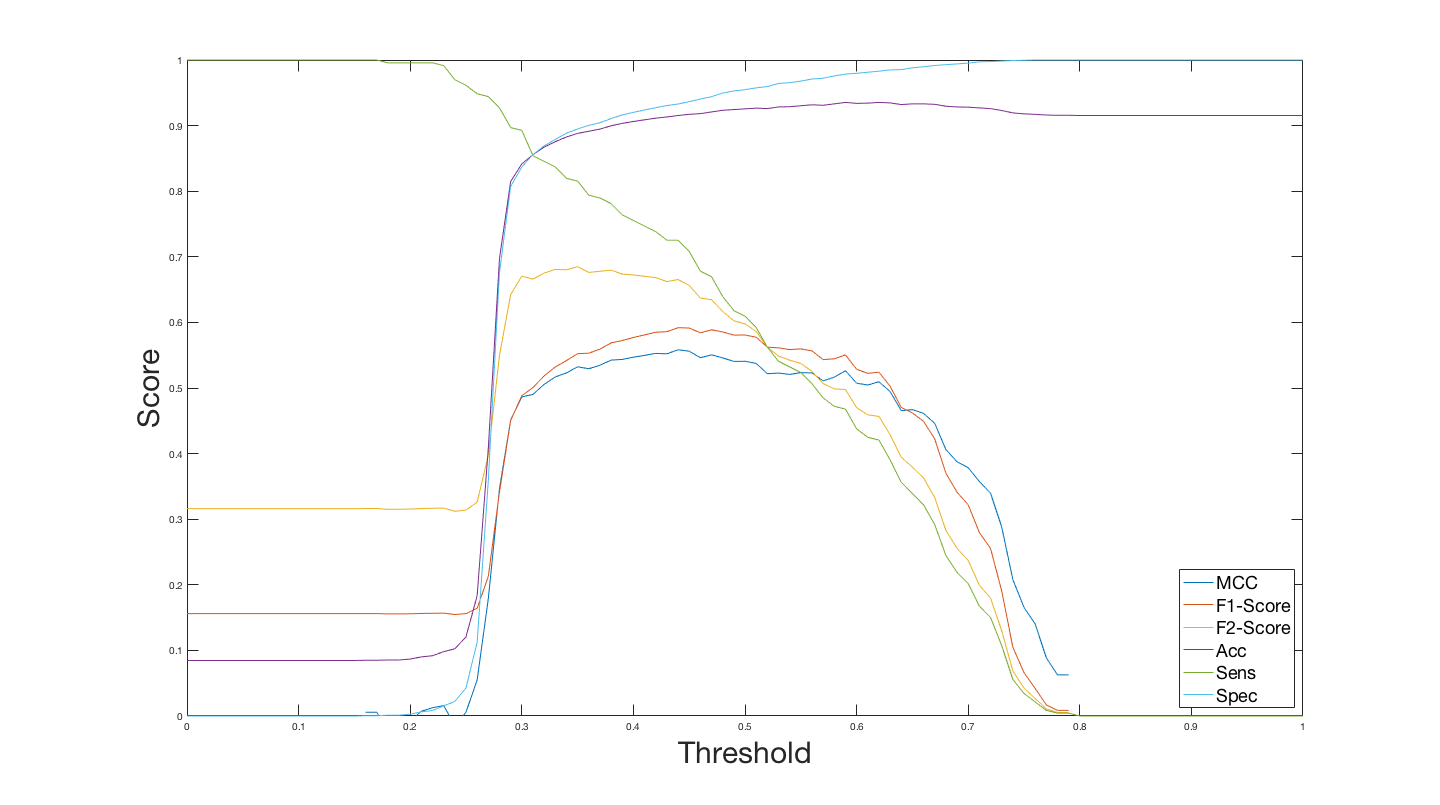
\includegraphics[width=0.8\textwidth]{pics/evaluation/treshold.png}
		\caption{Score-Threshold Abhängigkeit}
		\label{fig:threshold}
    \end{center}
\end{figure}

Wie man der Abbildung entnehmen kann, gibt es einen Bereich zwischen $0.3$ und $0.6$ in der der MCC und der F2-Score gute Werte aufweisen. Da der F2-Score die falsch negativen Stichproben noch stärker bestraft, konzentrierten wir uns hier mehr auf diesen Qualitätsmaßstab. Außerdem wollten wir eine möglichst hohe Sensitivität erreichen. Der F2-Score weist im Bereich $0.3$ und $0.45$ seine höchsten Werte auf, wobei der kleinste Threshold gleichzeitig die höchste Sensitivität liefert. Es wäre also naheliegend gewesen einfach diesen Wert zu nehmen. Da die Spezifität zwischen dem Threshold $0.25$ und $0.3$ rapide ansteigt, sollte allerdings ein gewisser Abstand zu diesem Bereich gewahrt werden. 

Abbildung~\ref{fig:verteilung} zeigt die Verteilung der Scores des Validierungsdatensatzes, der durch 2018-03-10\_19-16-32 klassifiziert wurde. Sie zeigt noch einmal deutlicher, dass die meisten benignen Stichproben einen Score zwischen $0.2$ und $0.3$ aufweisen. Somit entschieden wir uns den Threshold von den ursprünglichen $0.5$ auf $0.35$ herunterzusetzen. Damit halten wir genug Abstand von der extremen Änderung der Spezifität, klassifizieren gleichzeitig aber deutlich mehr maligne Stichproben richtig, ohne zu viele Fehler bei den negativen Stichproben zu machen. 

\begin{figure}[htb!]
	\begin{center}
		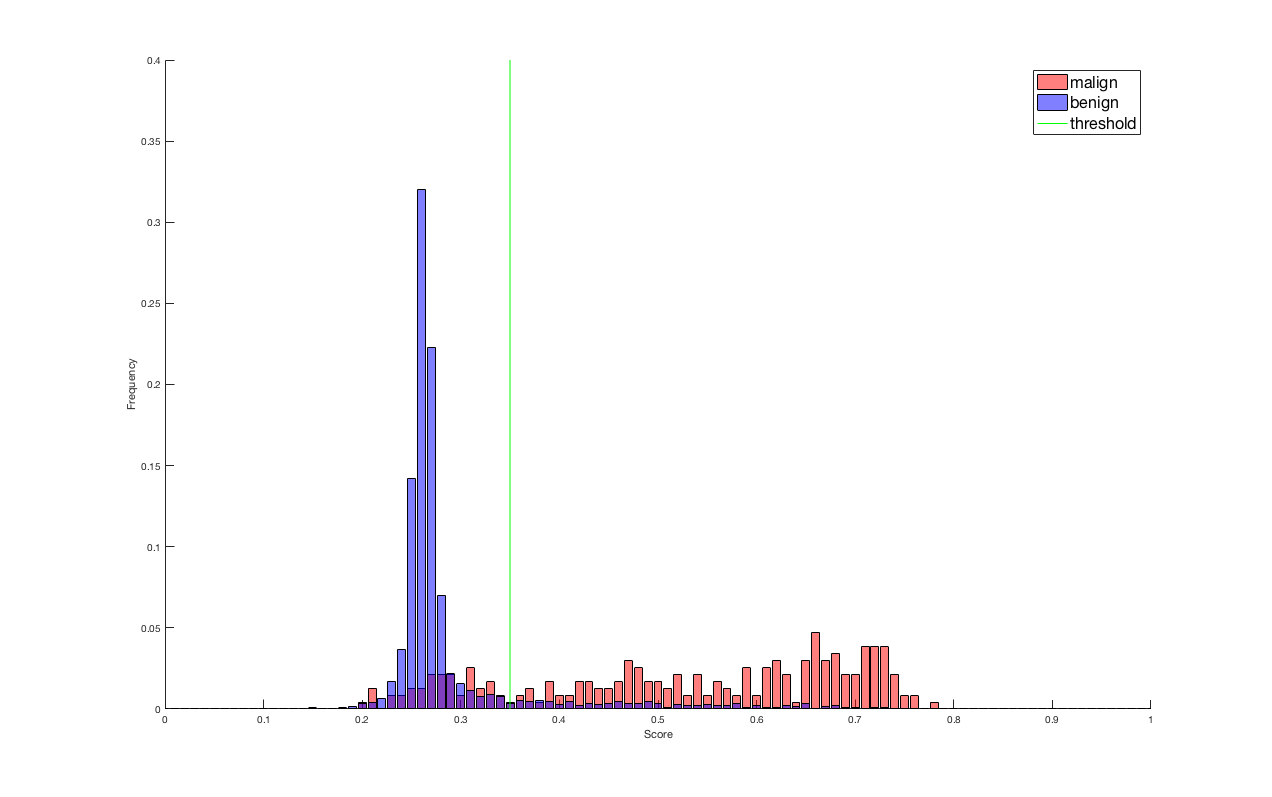
\includegraphics[width=0.8\textwidth]{pics/threshold/score_threshold.png}
		\caption{Verteilung der Vorhersagen auf dem Validierungsdatensatz. Maligne Stichproben werden in rot und benigne Stichproben in blau dargestellt. Die grüne Linie stellt den gewählten Threshold dar. Alle Vorhersagen links des Thresholds werden als benigne und alle Vorhersagen rechts des Thresholds werden als maligne klassifiziert.}
		\label{fig:verteilung}
    \end{center}
\end{figure}


Durch diese nun sensitivere Klassifizierung erhielten wir schließlich die Werte, wie sie in Tabelle~\ref{tab:final_scores} gelistet sind. Die Sensitivität konnten wir durch die Verschiebung des Thresholds von $0.61$ auf $0.81$ erhöhen. Es werden also nur noch zwei von zehn maligne Hautläsionen fälschlicherweise benigne klassifiziert. Dabei akzeptierten wir eine Verringerung der Spezifität von $0.95$ auf $0.89$. Es wird also etwa jede zehnte benigne Hautläsion falsch als maligne klassifiziert. Die Genauigkeit verringerte sich dabei von $93\%$ auf $89\%$, allerdings erhöhten wir den F2-Score von $0.6$ auf $0.68$, der bei einem unausgeglichenen Datensatz höher zu gewichten ist als die Gesamtgenauigkeit.

\begin{table}[htb!]
\begin{center}
\begin{tabular}{lllllllllll}
	\toprule
 	Threshold  & TP & FN & TN & FP & MCC & F2 & Acc & Sens & Spez\\
	\midrule
    $0.5$ & $142$&	$91$ &	$2406$ &	$114$ &	$0.54$ 	&$0.60$	&$0.93$	&$0.61$&	$0.95$ \\
	$0.35$ & $190$ & $43$ &	$2255$ &	$265$ &	$0.55$ &	$0.68$&	$0.89$ &	$0.81$ & $0.89$\\
 \bottomrule
 \end{tabular}
 \end{center}
  \caption{Scores des Klassifikators mit dem Threshold bei $0.35$}
 \label{tab:final_scores}
 \end{table}

Unser bester Klassifikator 2018-03-10\_19-16-32 wurde mit einer Batchsize von sechs sowie einer Lernrate von $e^{-0.6}$ trainiert. Als Loss-Funktion verwendeten wir das L2-Loss. Als Entscheidungsschranke nahmen wir, wie oben beschrieben, $0.35$. Dies bedeutet, dass alle Stichproben, die einen Score von über $0.35$ erhalten, als maligne Hautläsionen eingestuft werden. Schließlich testeten wir unseren finalen Prädiktor noch auf unserem Testdatensatz. Dieser Datensatz wurde bis an diese Stelle isoliert aufbewahrt und keine der enthaltenen Daten waren dem Klassifikator bekannt. Dies war nötig, um zu testen, ob dieser auch generalisierbar ist. Das bedeutet, dass dieser nicht nur die Trainingsdaten auswendig gelernt hat, sondern auch auf nie gesehenen Daten gute Vorhersagen macht. Da wir anhand des Validierungsdatensatzes schon die Trainingsparameter angepasst haben, wurde dieser Testdatensatz jetzt am Schluss verwendet, um die endgültige Performance zu testen. Tabelle~\ref{tab:test_scores} zeigt die Qualitätsmaßstäbe, wie sie auf dem finalen Testdatensatz berechnet wurden.

\begin{table}[htb!]
\begin{center}
\begin{tabular}{lllllllllll}
	\toprule
 	TP & FN & TN & FP & MCC & F2 & Acc & Sens & Spez\\
	\midrule
    $149$&	$60$ &	$2285$ &	$114$ &	$0.48$ 	&$0.60$	&$0.88$	&$0.71$&	$0.9$ \\
 \bottomrule
 \end{tabular}
 \end{center}
  \caption{Qualität des Klassifikators nach Anwendung auf ungesehenen Trainingsdatensatz, mit der Entscheidungsgrenze bei $0.35$}
 \label{tab:test_scores}
 \end{table}

 Wie zu erwarten sind die Ergebnisse ähnlich, aber etwas schlechter als auf dem Validierungsdatensatz, auf dem wir gezielt auf gute Werte hingearbeitet haben. Letzten Endes erkennt unser Prädiktor $90\%$ der benignen Hautläsionen richtig und $71\%$ der malignen Hautläsionen. Der F2-Score ist mit $0.6$ auch etwas gesunken, was an den häufigeren falsch negativen Vorhersagen liegt.

Zusammenfassend kann man sagen, dass diese Werte auf jeden Fall in einem guten Bereich liegen. Die drei von zehn falsch negativen Vorhersagen sind zwar nicht erwünscht, aber auch durch den unausgeglichenen Datensatz zu begründen. Mit mehr malignen Trainingsdaten wären womöglich noch bessere Vorhersagen möglich. Nichtsdestotrotz erhielten wir nach unzähligen Trainings einen Prädiktor, der mit Vorsicht zur häuslichen Vorsorge verwendet werden kann und akzeptable Vorhersagen für die Hautkrebserkennung liefert.


